\documentclass[11pt,a4paper]{article}

% Packages
\usepackage[utf8]{inputenc}
\usepackage[T1]{fontenc}
\usepackage[margin=2.5cm]{geometry}
\usepackage{amsmath,amssymb}
\usepackage{enumitem}
\usepackage{listings}
\usepackage{xcolor}
\usepackage{tikz}
\usetikzlibrary{shapes.geometric, arrows, positioning, calc}
\usepackage{fancyhdr}
\usepackage{lastpage}
\usepackage{array}
\usepackage{tabularx}
\usepackage{booktabs}

% Code listing style
\definecolor{codebg}{RGB}{248,248,248}
\definecolor{codeframe}{RGB}{200,200,200}
\definecolor{codekw}{RGB}{0,0,180}
\definecolor{codecomment}{RGB}{0,128,0}
\definecolor{codestring}{RGB}{163,21,21}

\lstdefinestyle{pythonstyle}{
    language=Python,
    basicstyle=\ttfamily\small,
    keywordstyle=\color{codekw}\bfseries,
    commentstyle=\color{codecomment}\itshape,
    stringstyle=\color{codestring},
    backgroundcolor=\color{codebg},
    frame=single,
    rulecolor=\color{codeframe},
    numbers=left,
    numberstyle=\tiny\color{gray},
    numbersep=8pt,
    showstringspaces=false,
    showlines=true,
    breaklines=true,
    tabsize=4,
    xleftmargin=15pt,
    framexleftmargin=15pt,
}

\lstset{style=pythonstyle}

% Flowchart styles
\tikzstyle{startstop} = [rectangle, rounded corners, minimum width=2.5cm, minimum height=0.8cm, text centered, draw=black, fill=red!20]
\tikzstyle{process} = [rectangle, minimum width=2.5cm, minimum height=0.8cm, text centered, draw=black, fill=blue!15]
\tikzstyle{decision} = [diamond, aspect=2, minimum width=2cm, minimum height=0.8cm, text centered, draw=black, fill=green!15]
\tikzstyle{io} = [trapezium, trapezium left angle=70, trapezium right angle=110, minimum width=2cm, minimum height=0.8cm, text centered, draw=black, fill=orange!15]
\tikzstyle{arrow} = [thick,->,>=stealth]

% Header and footer
\pagestyle{fancy}
\fancyhf{}
\lhead{Python Programming -- Third Chance Exam}
\rhead{}
\cfoot{Page \thepage\ of \pageref{LastPage}}

% Points box
\newcommand{\pointsbox}[1]{\hfill\fbox{\textbf{#1 pts}}}

\begin{document}

% Title section
\begin{center}
    {\Large\bfseries Python Programming}\\[0.3cm]
    {\large Third Chance Exam}\\[0.3cm]
    {\normalsize 28.02.2026}\\[0.5cm]

    \vfil
    \textbf{Name:} \hrulefill
    \vfil

\end{center}

\vspace{0.5cm}

\noindent\textbf{Instructions:}
\begin{itemize}[noitemsep]
    \item Time allowed: \textbf{2 hours}
    \item Total points: \textbf{60 points}
    \item No aids (no notes, no electronic devices)
\end{itemize}

\vspace{0.3cm}

\noindent\textbf{Points Summary:}
\begin{center}
    \begin{tabular}{|c|c|c|}
        \hline
        \textbf{Question} & \textbf{Max Points} & \textbf{Score} \\
        \hline
        1                 & 4                   &                \\
        \hline
        2                 & 6                   &                \\
        \hline
        3                 & 5                   &                \\
        \hline
        4                 & 7                   &                \\
        \hline
        5                 & 8                   &                \\
        \hline
        6                 & 6                   &                \\
        \hline
        7                 & 9                   &                \\
        \hline
        8                 & 15                  &                \\
        \hline
        \textbf{Total}    & \textbf{60}         &                \\
        \hline
    \end{tabular}
\end{center}

\newpage

%==============================================================================
% QUESTION 1: Multiple Choice (Fundamentals & Types)
%==============================================================================
\section*{Question 1: Multiple Choice \pointsbox{4}}

\textit{Circle the correct answer for each question. Each correct answer is worth 1 point.}

\vspace{0.4cm}

\begin{enumerate}[label=\textbf{1.\arabic*}]
    \item What is the output of the following expression?
          \begin{lstlisting}[numbers=none]
result = 29 // 4
print(result)
    \end{lstlisting}
          \begin{enumerate}[label=\Alph*)]
              \item \texttt{7.25}
              \item \texttt{7}
              \item \texttt{8}
              \item \texttt{1}
          \end{enumerate}

          \vspace{0.5cm}

    \item Which of the following is an \textbf{immutable} data type in Python?
          \begin{enumerate}[label=\Alph*)]
              \item \texttt{list}
              \item \texttt{dict}
              \item \texttt{tuple}
              \item \texttt{set}
          \end{enumerate}

          \vspace{0.5cm}

    \item What will \texttt{type(True)} return?
          \begin{enumerate}[label=\Alph*)]
              \item \texttt{<class 'int'>}
              \item \texttt{<class 'str'>}
              \item \texttt{<class 'bool'>}
              \item \texttt{<class 'binary'>}
          \end{enumerate}

          \vspace{0.5cm}

    \item What does the \texttt{super()} function do in a subclass?
          \begin{enumerate}[label=\Alph*)]
              \item Creates a new instance of the subclass
              \item Calls a method from the parent class
              \item Deletes the parent class
              \item Makes the subclass a global class
          \end{enumerate}
\end{enumerate}

\newpage

%==============================================================================
% QUESTION 2: Predict the Output
%==============================================================================
\section*{Question 2: Predict the Output \pointsbox{6}}

\textit{For each code snippet, write exactly what will be printed. Be precise with spacing and format.}

\vspace{0.4cm}

\begin{enumerate}[label=\textbf{2.\arabic*}]
    \item \textbf{(1 pt)}
          \begin{lstlisting}
words = ["red", "green", "blue", "yellow", "white"]
print(words[2:5])
print(words[-3])
    \end{lstlisting}
          \textbf{Output:}
          \vfil

    \item \textbf{(2 pts)}
          \begin{lstlisting}
p = 8
q = 5
p, q = p - q, p + q
print(f"p={p}, q={q}")
    \end{lstlisting}
          \textbf{Output:}


          \newpage
    \item \textbf{(1 pt)}
          \begin{lstlisting}
inventory = {"apples": 12, "bananas": 0, "oranges": 7}
for item in inventory:
    if inventory[item] > 0:
        print(item, end=" ")
    \end{lstlisting}
          \textbf{Output:}
          \vfil

    \item \textbf{(2 pts)}
          \begin{lstlisting}
def update(data):
    data["x"] = 99
    data = {"a": 1}
    return data

original = {"x": 10, "y": 20}
result = update(original)
print(original)
print(result)
    \end{lstlisting}
          \textbf{Output:}
          \vfil
\end{enumerate}

\newpage

%==============================================================================
% QUESTION 3: Find the Errors
%==============================================================================
\section*{Question 3: Find and Fix the Errors \pointsbox{5}}

\textit{Each code snippet contains one or more errors. Identify each error and write the corrected line(s). Explain briefly what was wrong.}

\vspace{0.4cm}

\begin{enumerate}[label=\textbf{3.\arabic*}]
    \item \textbf{(1 pt)} The following code should print the length of a list but contains an error:
          \begin{lstlisting}
items = [10, 20, 30]
size = len[items]
print(size)
    \end{lstlisting}
          \textbf{Error:}
          \vspace{3cm}

          \textbf{Correction:}
          \vfil

    \item \textbf{(2 pts)} The following function should return the largest number in a list:
          \begin{lstlisting}
def find_max(numbers):
    biggest = numbers[0]
    for num in numbers
        if num > biggest
            biggest = num
    return biggest
    \end{lstlisting}
          \textbf{Errors (list all):}
          \vspace{3cm}

          \textbf{Corrected code:}
          \vfil
          \newpage
    \item \textbf{(2 pts)} The following class definition has an error:
          \begin{lstlisting}
class Student:
    def __init__(self, name, grade):
        name = name
        grade = grade

s1 = Student("Alice", 90)
print(s1.name)
    \end{lstlisting}
          \textbf{Error:}
          \vspace{3cm}

          \textbf{Correction:}
          \vspace{1.5cm}
\end{enumerate}

\newpage

%==============================================================================
% QUESTION 4: Flowchart to Code
%==============================================================================
\section*{Question 4: Flowchart to Python Code \pointsbox{7}}

\textit{Study the following flowchart and write the equivalent Python code. The flowchart takes a positive integer and counts the number of even digits it contains.}

\vspace{0.4cm}

\begin{center}
    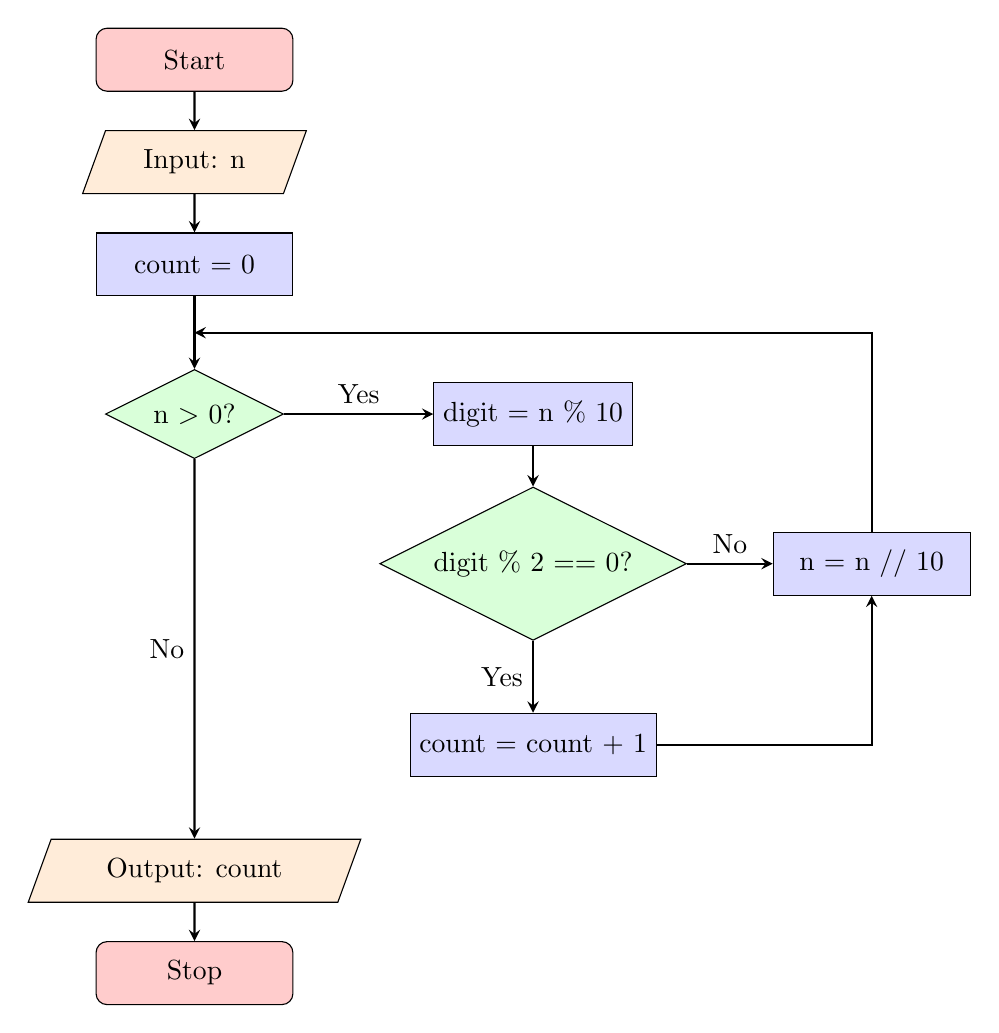
\begin{tikzpicture}[node distance=1.3cm]
        \node (start) [startstop] {Start};
        \node (input) [io, below of=start] {Input: n};
        \node (init) [process, below of=input] {count = 0};
        \node (check) [decision, below of=init, yshift=-0.6cm] {n $>$ 0?};
        \node (getdigit) [process, right of=check, xshift=3cm] {digit = n \% 10};
        \node (evencheck) [decision, below of=getdigit, yshift=-0.6cm] {digit \% 2 == 0?};
        \node (increment) [process, below of=evencheck, yshift=-1cm] {count = count + 1};
        \node (reduce) [process, right of=evencheck, xshift=3cm] {n = n // 10};

        \node (output) [io, below of=check, yshift=-4.5cm] {Output: count};
        \node (stop) [startstop, below of=output] {Stop};

        \draw [arrow] (start) -- (input);
        \draw [arrow] (input) -- (init);
        \draw [arrow] (init) -- (check);
        \draw [arrow] (check) -- node[anchor=south] {Yes} (getdigit);
        \draw [arrow] (getdigit) -- (evencheck);
        \draw [arrow] (evencheck) -- node[anchor=east] {Yes} (increment);
        \draw [arrow] (evencheck) -- node[anchor=south] {No} (reduce);
        \draw [arrow] (increment.east) -| (reduce.south);
        % Loop back
        \coordinate (loopback) at ($(init.south)!0.5!(check.north)$);
        \draw [arrow] (reduce.north) |- (loopback);
        \draw [arrow] (check) -- node[anchor=east] {No} (output);
        \draw [arrow] (output) -- (stop);
    \end{tikzpicture}
\end{center}

\vspace{0.3cm}
\textbf{Hint:} Trace through the flowchart with \texttt{n = 2483} to understand what it does before writing the code.

\vspace{0.2cm}
\textbf{Reminder:} \texttt{\%} gives the remainder, \texttt{//} gives the integer quotient.\\
\textit{Example:} \texttt{2483 \% 10 = 3} \quad and \quad \texttt{2483 // 10 = 248}

\vspace{0.3cm}
\textbf{Write the Python code that implements this flowchart on the next page.}

\newpage

\textbf{Question 4 -- Answer Space:}

\vfill

\newpage

%==============================================================================
% QUESTION 5: Code to Flowchart
%==============================================================================
\section*{Question 5: Python Code to Flowchart \pointsbox{8}}

\textit{Given the following Python code, draw a flowchart that represents its logic. Use proper flowchart symbols (oval for start/stop, rectangle for process, diamond for decision, parallelogram for input/output).}

\vspace{0.4cm}

\begin{lstlisting}
def evaluate_password(password):
    length = len(password)
    
    if length < 6:
        strength = "Weak"
    elif length < 10:
        has_digit = False
        for char in password:
            if char.isdigit():
                has_digit = True
        if has_digit:
            strength = "Medium"
        else:
            strength = "Weak"
    else:
        strength = "Strong"
    
    return strength
\end{lstlisting}

\vspace{0.3cm}
\textbf{Draw your flowchart on the next page.}

\newpage

\textbf{Question 5 -- Answer Space:}

\vfill

\newpage

%==============================================================================
% QUESTION 6: Data Structures
%==============================================================================
\section*{Question 6: Data Structures \pointsbox{6}}

\begin{enumerate}[label=\textbf{6.\arabic*}]
    \item \textbf{(2 pts)} Given the following dictionary, write Python code to:
          \begin{lstlisting}[numbers=none]
temperatures = {
    "Monday": 22,
    "Tuesday": 18,
    "Wednesday": 25,
    "Thursday": 20
}
    \end{lstlisting}

          \begin{enumerate}[label=\alph*)]
              \item Add ``Friday'' with a temperature of 27:
                    \vspace{1.5cm}

              \item Print all days where the temperature is above 21:
                    \vspace{2.5cm}
          \end{enumerate}

    \item \textbf{(2 pts)} What is the difference between a \textbf{dictionary} and a \textbf{list}? Give one practical use case for each.
          \vspace{3.5cm}

    \item \textbf{(2 pts)} What will be the contents of \texttt{colors} after executing the following code?
          \begin{lstlisting}
colors = {"red", "blue", "green", "blue", "red", "yellow"}
colors.add("purple")
colors.add("red")
colors.discard("green")
    \end{lstlisting}
          \textbf{Answer:}
          \vspace{1.5cm}
\end{enumerate}

\newpage

%==============================================================================
% QUESTION 7: Functions
%==============================================================================
\section*{Question 7: Functions \pointsbox{9}}

\begin{enumerate}[label=\textbf{7.\arabic*}]
    \item \textbf{(3 pts)} Complete the following function that takes a list of strings and returns a new list containing only the strings that have more than 4 characters:
          \begin{lstlisting}
def filter_long_words(words):
    # Your code here
 
 
 
 
 
 
 
 
 
 
 
 
 
 

    \end{lstlisting}
          \vfil
    \item \textbf{(3 pts)} Explain the difference between these two functions. What will each print when called?
          \begin{lstlisting}
def greet_a(name):
    return f"Hello, {name}!"

def greet_b(name):
    print(f"Hello, {name}!")

result_a = greet_a("Alice")
result_b = greet_b("Alice")
print(f"result_a: {result_a}")
print(f"result_b: {result_b}")
    \end{lstlisting}
          \textbf{Explanation and Output:}
          \vfil

          \newpage
    \item \textbf{(3 pts)} Write a function called \texttt{sum\_digits} that takes a positive integer and returns the sum of its digits.

          \textbf{Example:} \texttt{sum\_digits(1234)} should return \texttt{10}

          \textbf{Hint:} Use \texttt{\%} and \texttt{//} operators to extract digits.

          \vspace{7cm}
\end{enumerate}

\newpage

%==============================================================================
% QUESTION 8: Object-Oriented Programming
%==============================================================================
\section*{Question 8: Object-Oriented Programming \pointsbox{15}}

\begin{enumerate}[label=\textbf{8.\arabic*}]
    \item \textbf{(4 pts)} What is the output of the following code? Explain why.
          \begin{lstlisting}
class TemperatureSensor:
    def __init__(self, min_temp, max_temp):
        self._min = min_temp
        self._max = max_temp
        self._reading = min_temp
    
    @property
    def reading(self):
        return self._reading
    
    @reading.setter
    def reading(self, value):
        if value < self._min:
            print("Below minimum! Clamping.")
            self._reading = self._min
        elif value > self._max:
            print("Above maximum! Clamping.")
            self._reading = self._max
        else:
            self._reading = value
    
    def status(self):
        mid = (self._min + self._max) / 2
        if self._reading >= mid:
            return "HIGH"
        return "LOW"

sensor = TemperatureSensor(0, 100)
sensor.reading = 75
print(sensor.reading)
print(sensor.status())
sensor.reading = 150
print(sensor.reading)
sensor.reading = -10
print(sensor.reading)
    \end{lstlisting}
          \textbf{Output:}
          \vspace{2.5cm}

          \textbf{What is the purpose of the setter validation in this code?}
          \vspace{2cm}

          \newpage
    \item \textbf{(4 pts)} The following code has a common OOP bug. Identify the bug, explain why it happens, and write the corrected code.
          \begin{lstlisting}
class ShoppingCart:
    items = []
    
    def __init__(self, customer):
        self.customer = customer
    
    def add_item(self, item):
        self.items.append(item)

cart1 = ShoppingCart("Alice")
cart2 = ShoppingCart("Bob")
cart1.add_item("Laptop")
cart2.add_item("Phone")
print(f"Alice: {cart1.items}")
print(f"Bob: {cart2.items}")
    \end{lstlisting}
          \textbf{What is the bug and why does it happen?}
          \vspace{2.5cm}

          \textbf{Write the corrected \texttt{\_\_init\_\_} method:}
          \vspace{4cm}

          \newpage

    \item \textbf{(4 pts)} Complete the \texttt{ContactBook} class with proper encapsulation. The contacts dictionary should be private (use \texttt{\_contacts}) and only accessible through a property that returns a copy (to prevent external modification).
          \begin{lstlisting}
class ContactBook:
    def __init__(self, owner):
        self.owner = owner
        # TODO: Initialize private _contacts as empty dict
 
 

    @property
    def contacts(self):
        # TODO: Return a COPY of the contacts dict
 
 

    @property
    def total_contacts(self):
        # TODO: Return number of contacts
 
 

    def add_contact(self, name, phone):
        # TODO: Add contact only if name not already in book
        # Return True if added, False if duplicate
 
 
 
 
 
 

    def remove_contact(self, name):
        # TODO: Remove contact if exists
        # Return True if removed, False if not found
 
 
 
 
 
 
    \end{lstlisting}

          \newpage
    \item \textbf{(3 pts)} Consider the following inheritance hierarchy:
          \begin{lstlisting}
class Shape:
    def __init__(self, color):
        self.color = color
    
    def describe(self):
        return f"Shape({self.color})"

class Rectangle(Shape):
    def __init__(self, color, width, height):
        super().__init__(color)
        self.width = width
        self.height = height
    
    def describe(self):
        base = super().describe()
        return f"{base}, {self.width}x{self.height}"

class Square(Rectangle):
    def __init__(self, color, side):
        super().__init__(color, side, side)
    
    def describe(self):
        base = super().describe()
        return f"{base}, Square"

s = Square("red", 5)
print(s.describe())
print(isinstance(s, Shape))
    \end{lstlisting}

          \begin{enumerate}[label=\alph*)]
              \item What will be printed?
                    \vspace{1.5cm}

              \item Trace the \texttt{super().describe()} calls: which methods are called and in what order when \texttt{s.describe()} executes?
                    \vspace{2cm}

              \item What would happen if \texttt{Square.\_\_init\_\_} did not call \texttt{super().\_\_init\_\_()}? Explain briefly.
                    \vspace{2cm}
          \end{enumerate}
\end{enumerate}

\vfill

\begin{center}
    \rule{8cm}{0.4pt}\\[0.3cm]
    \textbf{End of Exam}\\[0.2cm]
    \textit{Good luck!}
\end{center}

\end{document}
